\documentclass[letterpaper]{article}
\usepackage{graphicx}
\usepackage{mathtools}
\usepackage{tabularx}
\usepackage{hyperref}
\usepackage{float}
\usepackage{parskip}
\usepackage{color,soul}
\usepackage{amsfonts}
\usepackage{pdfpages}
\usepackage{xfrac}
\usepackage{fix-cm}
\usepackage{bookmark}
\usepackage{listings}
\usepackage{framed}
\usepackage{makecell}
\usepackage[margin=1.5in]{geometry}
\usepackage[dvipsnames]{xcolor}
\setlength{\parskip}{1em}
\parindent=0pt

\title{ESE5400: Case Study \#1}
\author{Calum Mitchell, Siddharth Ramanathan, Vishnu Venkatesh}
\date{October 2024}

\begin{document}

\maketitle

The risk-free rate should be the same one as the expected investment horizon - a typical value of 10 years should be the one we consider, so the risk free rate that we are using in the CAPM model is 4.66\%. With $r_f = 4.66\%$, we can compute the cost of debt $r_D$ and the cost of equity $r_E$.

For the consolidated company, Midland's pre-tax cost of debt can be computed from the risk-free rate $r_f$ and the spread to treasury.

\begin{table}[H]
    \begin{tabularx}{\textwidth}{|>{\centering\arraybackslash}X|>{\centering\arraybackslash}X|>{\centering\arraybackslash}X|>{\centering\arraybackslash}X|}
        \hline
        Business Segment & Credit Rating & Spread to Treasury & Cost of debt \\ \hline
        Consolidated & A+ & 1.62\% & 6.28\%\\ \hline
        Exploration \& Production & A+ & 1.60\% & 6.26\%\\ \hline
        Refining \& Marketing & BBB & 1.80\% & 6.46\% \\ \hline
        Petrochemicals & AA- & 1.35\% & 6.01\% \\ \hline
    \end{tabularx}
\end{table}

The cost of debt (before tax) would be for the consolidated company, so

\[
r_D = 6.28\%
\]

These 4 costs of debt are different because the credit ratings correspond with the perceived amount of risk involved in the debt. For example, a rating of BBB is the lowest credit rating on the table and we see that it has the highest spread (and therefore the highest cost of debt) of 1.80\% compared to the other business segments in the table. Conversely, AA- is the highest credit rating and therefore the least risky to loan money to - and we see that it has a correspondingly lower spread than any other business segment at 1.35\%. 

We can also analyze the difference in the 4 costs of debt based on the nature of operations. Refining \& Marketing is seen as a riskier venture to invest in for three reasons: (a) stiff competition; (b) highly commoditized products; and (c) declining margins over the previous 20 years. So Refining \& Marketing has the lowest credit rating and therefore the highest cost of debt. Exploration \& Production was one of Midland's most profitable ventures, so there is a little more confidence in that business venture. However, that is offset by the fact that Midland has assets in politically volatile regions like the Middle East, Central Asia, Russia, and West Africa. So it has a slightly higher credit rating of A+. Petrochemicals has the highest credit rating because it has manufacturing facilities and research centers all over the world. Several older facilities were also replaced by more efficient ones - so there is much more confidence in this business segment compared to the other two, and that reflects in the highest credit rating out of the three (AA-) and the lowest cost of debt (6.01\%).

For Midland's WACC calculations, we care about the WACC in year 2006. So it makes the most sense to take the tax in year 2006.

\begin{align*}
    t_{2006} = \frac{Taxes \;Charged}{Income\; Before\; Taxes} = \frac{\$11,747}{\$30,447} = 38.58\% \\
\end{align*}

So the average tax rate that we recommend using for WACC calculations is 38.58\%.

The EMRP represents the difference between the expected return of a diversified portfolio and the risk-free rate. 

\[
\text{EMRP} = \text{Expected Portfolio Return} - \text{Risk-Free Rate}
\]

An EMRP of 5\% implies an expected diversified portfolio return will be 4.66\% + 5\% = 9.66\%. We can use this to estimate Midland's consolidated cost of equity using the formula below.

\[
r_E = r_f + \beta \times \text{EMRP}
\]

We can get the value of $\beta$ from Exhibit 5 -- the equity beta is given to be 1.25. Using this, we can calculate Midland's consolidated cost of equity:

\begin{align*}
r_E &= 4.66\% + 1.25 \times 5\% \\
r_E &= 10.91\%
\end{align*}

Regarding Midland's after-tax cost of capital, we need one more piece of information -- the debt fraction of total capital, $\lambda$. We see from Exhibit 5 that the D/E ratio is 59.3\%:

\begin{align*}
    \lambda &= \frac{D}{D+E} \\
            &= \frac{\frac{D}{E}}{\frac{D}{E} + 1} \\
            &= \frac{0.593}{0.593 + 1} \\
            &= \frac{0.593}{1.593} \\
    \lambda &= 37.23\%
\end{align*}
\begin{align*}
WACC_{a.t.} &= \lambda (1-t) r_D + (1-\lambda)r_E \\
            &= 0.3723 \times (1 - 0.3858) \times 0.0628 + (1 - 0.3723) \times 0.1091 \\
            &= 0.08285
\end{align*}

Midland's $WACC_{a.t.}$ is 8.29\%.

To find the un-levered asset beta, we can use the formula below:

\begin{align*}
\beta_{\text{Asset}} &= \frac{\text{Equity}}{\text{Debt + Equity}}\times \beta_{\text{Equity}} \\
                    &= (1 - \lambda) \times \beta_{\text{Equity}} \\
                    &= (1 - 0.3723) \times 1.25 \\
                    &= 0.78468
\end{align*}

The un-levered asset beta ($\beta_{Asset}$) is 0.785.

The analysis so far has been done with data from 2006. Exhibit 5 mentions that the data is for EOY 2006. Table 1 indicates the target debt ratios for 2007 - we see that the target debt value is 42.2\%. This is a slight increase from the original debt value of 37.23\% so we must recalculate our beta using this new value:

\begin{align*}
\lambda_{1} &= 0.3723 \\
\lambda_{2} &= 0.422  \\
\beta_{Asset} &= (1 - \lambda_{1}) \times \beta_{Equity} \\
            &= 0.785 \\
\beta_{Equity,2} &= \frac{1}{1-\lambda_{2}} \times \beta_{Asset} \\
                &= \frac{1}{1-0.422} \times 0.785 \\
                &= 1.3576
\end{align*}

We can use this new value of beta to compute the future cost of equity.

\begin{align*}
r_{E,2} &= r_f + \beta_{Equity, 2} \times \text{EMRP} \\
    &= 0.0466 + 1.3576 * 0.05 \\
    &= 0.114479
\end{align*}

We find a new cost of equity of 11.45\%. The corresponding WACC can be calculated as shown below:

\begin{align*}
WACC_{a.t., 2007} &= \lambda_2 (1-t) r_D + (1-\lambda_2)r_{E,2} \\
            &= 0.422 \times (1 - 0.3858) \times 0.0628 + (1 - 0.422) \times 0.1145 \\
            &= 0.08244
\end{align*}

The corresponding WACC is 8.24\%. This is lesser than the WACC in 2006 by 0.05\%. A lower WACC implies that the company can more easily acquire financing for any project it wants to take on, which means there are more economically viable investments that the company can undertake.

To graph the company's cost of equity and WACC as a function of it debt fraction, we can unlever and relever the beta values for each debt fraction and plot the corresponding costs of equity and WACC.

\begin{figure}[H]
    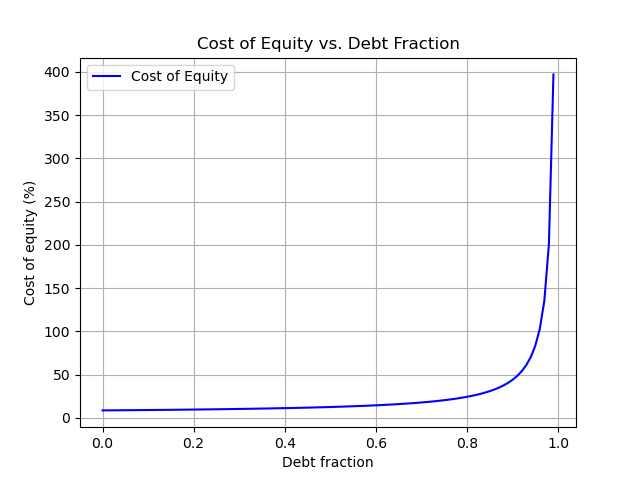
\includegraphics[width=\linewidth]{images/cost_of_equity.png}
    \caption{Cost of equity vs. Debt Fraction}
\end{figure}

The cost of equity rises because as the debt fraction increases, the risk to investors increases so they demand a higher rate of return. At zero debt, there is little risk to investors -- so the cost of equity is very low. As debt increases, the return that the investors require increases as well. As debt fraction approaches one, the amount of debt approaches the amount of value or collateral of a company, meaning the company almost has more debt than the market value of its assets, making it an extremely risky investment, hence the exponential increase to cost of equity. 
\color{black}

\begin{figure}[H]
    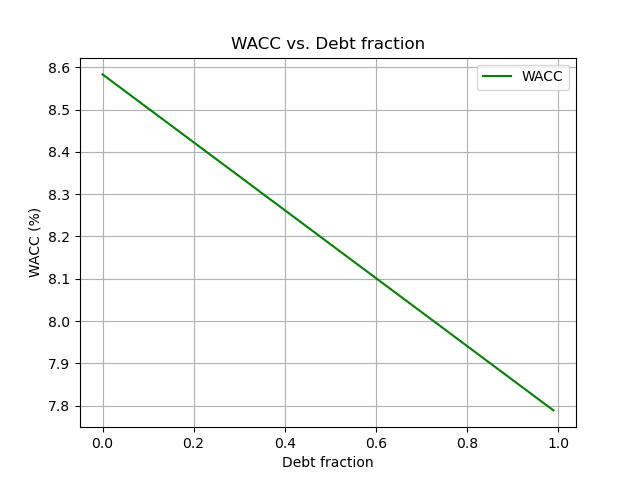
\includegraphics[width=\linewidth]{images/wacc.png}
    \caption{WACC vs. Debt Fraction}
\end{figure}

This ties with our WACC formula because as the proportion of debt to value increases, the equity term in the formula will decrease. Since we assume a constant cost of debt, this leads to a decreasing linear relationship. In a macro view, WACC is expected to eventually begin increasing again as the risk of debt grows because both lenders and equity holders will require greater returns. 

In a practical sense, the optimal debt fraction for a company should be in between the two extremes. Investors generally do not want to invest in a company that either does not offer satisfactory rates of return or is too risky. Midland, being an energy company, will have to take on debt to finance oil exploration, well drilling, and other expensive projects. However, it should not want to increase its cost of debt too much as that would increase its cost of equity and financial risk. Midland should avoid too low of a WACC which would indicate an over-reliance on debt financing but too high of a WACC would limit investment opportunities and make projects less affordable. 

\begin{table}[H]
    \begin{tabularx}{\textwidth}{|>{\centering\arraybackslash}X|>{\centering\arraybackslash}X|>{\centering\arraybackslash}X|>{\centering\arraybackslash}X|}
        \hline
         & Asset Beta \\ \hline
        \textit{Exploration \& Production:} & \\ \hline
        Jackson Energy, Inc. & 0.80 \\ \hline
        Wide Plain Petroleum & 0.65\\ \hline
        Corsicana Energy Corp. & 0.96\\ \hline
        Worthington Petroleum & 0.94\\ \hline
        \textbf{Average}& \textbf{.84}\\ \hline
        & \\ \hline
        \textit{Refining \& Marketing:} & \\ \hline
        Bexar Energy, Inc. & 1.54\\ \hline
        Kirk Corp. & .79\\ \hline
        White Point Energy & 1.47\\ \hline
        Arkana Petroleum Corp. & .94\\ \hline
        Beaumont Energy, Inc. & .86\\ \hline
        Dameron Fuel Services & .94\\ \hline
        \textbf{Average} & \textbf{1.09}\\ \hline
    \end{tabularx}
\end{table}
Using the same equations as previous calculations, we can unlever and relever the averages in the table above to find the equity betas for both Midland's Exploration \& Production and Refining \& Marketing divisions:
\begin{align*}
    \text{Exploration \& Production}\; \beta_E = 1.56\\
    \text{Refining \& Marketing}\; \beta_E = 1.58 
\end{align*}
Similarly, we can find each division's cost of equity and WACC:
\begin{align*}
    \text{Exploration \& Production}\; r_E = 12.4\%\\
    \text{Exploration \& Production}\; \text{WACC} = 8.5\%\\
    \text{Refining \& Marketing}\; r_E = 12.6\%\\
    \text{Refining \& Marketing}\; \text{WACC} = 9.9\%
\end{align*}
If these new WACC hurdles were used, Midland would require a greater return on investment for investments within the Refining and Marketing division. This result ties with our comparable asset betas, with a value greater than one for companies in refining and marketing, implying that they are riskier or more volatile. Therefore, Midland's investment decisions within this division should be more careful and inquire deeper into potential gains and risk management to better reflect Midland's comparables. 

Subsequently, Midland should use differing hurdle rates for each division because the Exploration and Production division is less risky on average, as shown in the table above. Midland's consolidated equity beta of 1.25 implies that the company as a whole is rather volatile but we now know that this is mostly due to its Refining and Marketing division. While using a consolidated WACC would be simpler from a management perspective, it would increase the cost of equity for one division unnecessarily. Differing hurdle rates allows for Midland to better understand its different businesses and to optimize its investment decisions according to each division's risk. 


\end{document}
